%%%%%%%%%%%%%%%%%%%%%%%%%%%%%%%%%%%%%%%%%%%%%%%%%%%%%%%%%%%%%%%%%%%
% Chapter 3: Method
%%%%%%%%%%%%%%%%%%%%%%%%%%%%%%%%%%%%%%%%%%%%%%%%%%%%%%%%%%%%%%%%%%%

\chapter{Methodology}
\label{chap:method}

% Phương pháp của chúng tôi bao gồm hai phần chính hoạt động song song nhau: (1) - Feature extraction; (2) - Model synthesis. Tổng quan phương pháp được minh họa trong hình \ref{fig:flow}. Trong phần feature extraction, chúng tôi kết hợp hai loại đặc trưng từ mạng \verb|BiLSTM| và \verb|LSTM+CNN|. Trong phần Model synthesis, chúng tôi sử dụng \verb|MAML| để tổng hợp tham số của các mô hình. Với sự góp mặt của các đặc trưng từ các mạng học sâu, chúng tôi kỳ vọng sẽ rút trích được các đặc trưng ẩn trong dữ liệu aperiodic. Thông qua sự kết hợp giữa quá trình tổng hợp mô hình bằng thuật toán \verb|MAML| và quá trình rút trích đặc trưng bằng \verb|BiLSTM|/\verb|LSTM+CNN|, phương pháp đề xuất được kỳ vọng là một giải pháp thay thế hợp lý và hiệu quả cho các mô hình ensemble truyền thống trong việc tổng hợp hiệu quả external factors, giảm thiểu tác động của sự biến thiên phương sai, cũng như rút trích được các hidden long-term dependency trong quá khứ.

We propose \verb|Temporal-ML|, a ML-based method which consists of two main components that work in parallel: (1) - Temporal feature extraction; (2) - Models' parameter synthesis. The overview of the method is illustrated in figure \ref{fig:flow} and the detail is presented in algorithm \ref{alg:maml}. In the \textit{Temporal feature extraction} section, we propose to use the features extracted from \verb|BiLSTM| network. In the \textit{Effective synthesis of model's parameters} section, \verb|MAML| is utilized to synthesize the parameters of the models.

Due to the contribution of \verb|BiLSTM| features, we expect to effectively extract hidden temporal features from aperiodic data. By using \verb|MAML| in the weight aggregation process, the proposed method is expected to be a reasonable and effective alternative to traditional ensemble models in effectively synthesizing external factors, minimizing the impact of variance variation, and efficiency capturing hidden long-term dependencies in the past.

\begin{figure}[H]
    \centering
    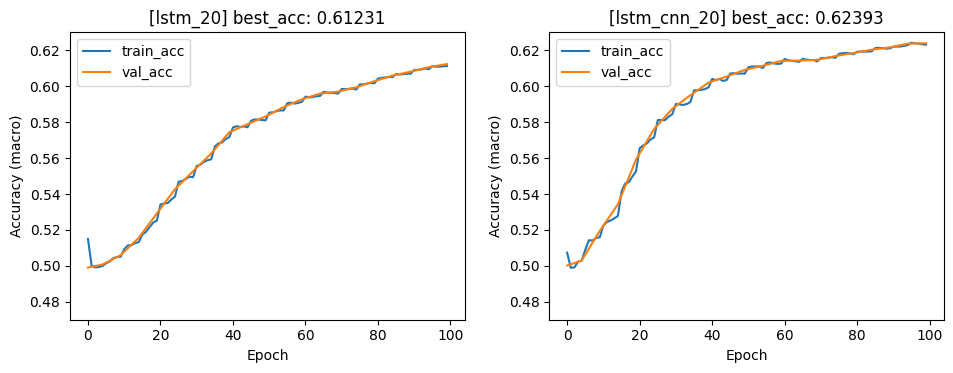
\includegraphics[width=\textwidth]{meta.png}
    \caption{The full-flow of meta-training and meta-testing on multi-fx data. Each currency pair is regarded as a task.}
    \label{fig:flow}
\end{figure}

\begin{algorithm}[H]
    \caption{Temporal-ML} \label{alg:maml}
    \begin{algorithmic}[1]
        \State Initialize $\phi_0$
        \For{round $r=1,2,...$} \Comment{Outer loop}
            \State Sample a subset $T_r$ of $m$ tasks
            \For{task $t \in T_r$} \Comment{Inner loop}
                \State Initialize inner weight $\theta_t^{(0)} \leftarrow \phi_{r-1}$
                \State Forward: For all data point $\mathbf{x}_{}$ in $\mathcal{D}_t^{support}$
                \begin{align*}
                    \mathbf{x'} &= \mathbf{FullyConnected}\left( \mathbf{x} \right)\\
                    \mathbf{h}_{LSTM} &= \mathbf{BiLSTM}\left( \mathbf{x'} \right)\\
                    \hat{y} &= \mathbf{FullyConnected}\left( \mathbf{h}_{LSTM} \right)
                \end{align*}

                \State Backward and aggregate meta loss:\Comment{Inner optimization}
                \begin{align*}
                    &\mathcal{L}_t^{task}\left( \theta_t^{(e-1)}, \mathcal{D}_t^{support} \right) = \mathbf{CrossEntropyLoss}\left( \mathbf{y}, \hat{\mathbf{y}} \right)\\
                    &\theta_t^{(e)} \leftarrow \theta_t^{(e-1)} - \alpha\nabla_\theta\mathcal{L}_t^{task}\left( \theta_t^{(e-1)}, \mathcal{D}_t^{support} \right)\\
                    &\mathcal{L}^{meta} \leftarrow \mathcal{L}^{meta} + \mathcal{L}_t^{meta}\left( \theta_t^{(e)}, \mathcal{D}_t^{query} \right)
                \end{align*}
            \EndFor

            \State Outer optimization at round $r$:\Comment{Outer optimization}
            \begin{align*}
                \phi_{r+1} \leftarrow \phi_r - \beta\nabla_\phi\mathcal{L}^{meta}
            \end{align*}
        \EndFor
    \end{algorithmic}
\end{algorithm}

\section{Data preparation}
\label{sec:data_prep}

% Phương pháp đề xuất sử dụng các thuật toán ML để huấn luyện mô hình. Do đó, dữ liệu cần được tổ chức lại để các thuật toán ML có thể hoạt động được. Trong trường hợp dữ liệu bao gồm nhiều datasets khác nhau thuộc cùng một lĩnh vực, mỗi dataset sẽ được coi là một task của \verb|MAML|. Trong trường hợp dữ liệu bao gồm một dataset duy nhất, cần chia nhỏ dataset này thành các tập con ứng với các task riêng biệt. Tóm lại, tập dữ liệu sau khi chuẩn bị bao gồm $n$ tasks: $\mathcal{D} = \left\{ \mathcal{D}_t \right\}_{t=1}^{n}$. Dữ liệu tại mỗi task được chia thành tập support và query: $\mathcal{D}_t = \left\{ \mathcal{D}_t^{support}, \mathcal{D}_t^{query} \right\}$.

\verb|Temporal-ML| uses ML algorithms to train the model. Therefore, the data must be reorganized so that the ML algorithms can work. In case the data includes many different datasets belonging to the same field, each dataset will be considered a task. \textbf{The goal of using multiple datasets of the same domain is to utilize the corelation between them} as indicated in study \cite{overreactioncontrarian, mech1993portfolio}. In case the data includes a single dataset, it is necessary to divide this dataset into subsets corresponding to separate tasks. \textbf{In this way, we aim to enhance the learning of information about external factor reflected in single dataset} \cite{fama1970efficient}. In summary, the prepared dataset includes $n$ tasks: $\mathcal{D} = \left\{ \mathcal{D}_t \right\}_{t=1}^{n}$. The data at each task is divided into support and query sets: $\mathcal{D}_t = \left\{ \mathcal{D}_t^{support}, \mathcal{D}_t^{query} \right\}$.

% Một sample dữ liệu bao gồm các cặp giá trị $(\mathbf{x}_{t-L:t}, y)$. Trong đó, $\mathbf{x}_{t-L:t}$ bao gồm $L$ giá trị lịch sử tính từ thời điểm $t$ trở về trước; $y\in \{0,1\}$ là nhãn dữ liệu, thể hiện xu hướng giảm, hoặc tăng của mẫu dữ liệu $x_{t+1}$ so với $x_{t}$. Tùy vào từng bài toán và cách cài đặt mà các phần tử trong $\mathbf{x}_{t-L:t}$ có thể là các vector hoặc các scalar number. Ví dụ, đối với dữ liệu chứng khoán, $\mathbf{x}_{t-L:t}$ có thể chứa các vector dữ liệu $\vec x_i = (\text{open, low, high, close})$ hoặc chỉ một giá trị close price duy nhất.

A data sample consists of pairs of values $(\mathbf{x}_{t-L:t}, y)$. In which, $\mathbf{x}_{t-L:t}$ includes $L$ historical values from time $t$ back; $y\in \{0,1\}$ is the data label, showing the decreasing or increasing trend of the data sample $x_{t+1}$ compared to $x_{t}$. Depending on each problem and the implementation, the elements in $\mathbf{x}_{t-L:t}$ can be a matrix or a vector. For example, for stock data, $\mathbf{x}_{t-L:t}$ can contain $L$ vectors $\vec x_i = (\text{open, low, high, close})$ or can be a vector of close price values only.

\section{Temporal feature extraction}

% Quá trình rút trích đặc trưng được thực hiện bằng hai phương pháp khác nhau: thông qua \verb|BiLSTM| và \verb|LSTM+CNN|. Đối với phương pháp sử dụng \verb|BiLSTM|, từng phần tử trong ma trận $\mathbf{x}_{t-L:t}$ (viết gọn là $\mathbf{x}$) được đưa qua một lớp \verb|FullyConnected| có đầu ra lớn hơn số chiều của $\vec x_i, i\in[t-L, t]$ to present the input by a larger vector $\vec x'_i$ (equation \ref{eq:decompose}). Theo đó, các đặc trưng được thể hiện sâu sắc và rõ ràng hơn. Các đặc trưng này sau đó được truyền qua mạng \verb|BiLSTM| rút trích có chọn lọc các phụ thuộc thời gian dài hạn ($\mathbf{h}_{LSTM}$). Để có thể khai thác tối đa các ràng buộc thời gian dài hạn, chúng tôi sử dụng \verb|BiLSTM| để rút trích từ hai phía của của $\mathbf{x}$ (equation \ref{eq:feature_lstm})

Feature extraction is performed using \verb|BiLSTM|. Specifically, each element in the matrix $\mathbf{x}_{t-L:t}$ (abbreviated as $\mathbf{x}$) is passed through a \verb|FullyConnected| layer whose output is larger than the dimension of $\vec x_i, i\in[t-L, t]$ to obtain vector $\vec x'_i$ (equation \ref{eq:decompose}). Accordingly, the data characteristics are expressed more deeply and clearly. These features are then passed through the \verb|BiLSTM| network (equation \ref{eq:feature_lstm}) to selectively extract long-term temporal dependencies ($\mathbf{h}_{BiLSTM}$). At the end, $\mathbf{h}_{BiLSTM}$ is passed through a classification head of the neural network (equation \ref{eq:clf}) to predict the label of $\mathbf{x}$.

\begin{align}
    \mathbf{x'} &= \mathbf{FullyConnected}\left( \mathbf{x} \right) \label{eq:decompose}\\
    \mathbf{h}_{BiLSTM} &= \mathbf{BiLSTM}\left( \mathbf{x'} \right) \label{eq:feature_lstm}\\
    \hat y &= \mathbf{FullyConnected}\left( \mathbf{h}_{BiLSTM} \right) \label{eq:clf}
\end{align}

% Lấy cảm hứng từ nghiên cứu \cite{vo2017multi}, chúng tôi đề xuất \verb|LSTM+CNN|, kết hợp các đặc trưng rút trích được từ mạng \verb|BiLSTM| và \verb|CNN|. Cụ thể, ngoài việc sử dụng \verb|BiLSTM|, $\mathbf{x'}$ còn được đưa vào \verb|CNN| để rút trích đặc trưng thời gian cục bộ ($\mathbf{h}_{CNN}$) (equation \ref{eq:feature_cnn}). Tiếp đến, $\mathbf{h}_{LSTM}$ và $\mathbf{h}_{CNN}$ được nối với nhau (equation \ref{eq:concat}) sau đó chuyển đến phần phân lớp của neural network (equation \ref{eq:clf}).

% Inspired by study \cite{vo2017multi}, we use \verb|LSTM+CNN| features, which combines the features extracted from \verb|BiLSTM| and \verb|CNN|. Specifically, in addition to using \verb|BiLSTM|, $\mathbf{x'}$ is also fed into \verb|CNN| to extract local temporal features $\mathbf{h}_{CNN}$ (equation \ref{eq:feature_cnn}). Next, $\mathbf{h}_{LSTM}$ and $\mathbf{h}_{CNN}$ are concatenated (equation \ref{eq:concat}) and then passed to the classification head of the neural network (equation \ref{eq:clf}).

% \begin{align}
%     \mathbf{h}_{CNN} &= \mathbf{Convolution1D}\left( \mathbf{x'} \right) \label{eq:feature_cnn}\\
%     \mathbf{h} &= \mathbf{Concatenate}\left( \mathbf{h}_{LSTM}, \mathbf{h}_{CNN} \right) \label{eq:concat} \\
%     \hat y &= \mathbf{FullyConnected}\left( \mathbf{h} \right) \label{eq:clf}
% \end{align}

% Mạng \verb|BiLSTM| duy trì giá trị cell-state nhằm lưu trữ có chọn lọc các phụ thuộc dài hạn. Điều này rất thích hợp trong việc giải quyết các bài toán time-series data. Mặt khác, giá trị tương lai thường phụ thuộc rất lớn vào các giá trị lịch sử gần nhất. Chúng tôi đề xuất sử dụng mạng \verb|CNN| để nhấn mạnh các đặc trưng cục bộ, từ đó hướng một phần sự chú ý của mô hình vào các thời điểm nhất định. Do đó, phương pháp đề xuất không chỉ nhớ được các đặc trưng long-term mà còn highlight được các đặc trưng short-term.

% The \verb|BiLSTM| network maintains cell-state values to selectively store long-term dependencies. Thus, this method is a suitable choice for solving time-series data problems. On the other hand, future values often depend heavily on recent historical values. We propose to use the \verb|CNN| network to emphasize local features, thereby directing part of the model's attention to certain time points. \textbf{Therefore, the proposed method not only remembers long-term features but also highlights short-term features. In the ideal situation, hidden constraints in aperiodic time-series data can be extracted efficiently}.

% The \verb|BiLSTM| network maintains cell-state values to selectively store long-term dependencies. Thus, this method is a suitable choice for solving time-series data problems. \textbf{Therefore, the proposed method not only remembers long-term features but also highlights short-term features. In the ideal situation, hidden constraints in aperiodic time-series data can be extracted efficiently}.

% Mạng \verb|LSTM| và \verb|BiLSTM| đều duy trì các giá trị cell-state để lưu trữ một cách chọn lọc các phụ thuộc thời gian, cũng như hạn chế vấn đề vanishing gradient trong quá trình huấn luyện. Vì vậy, các mạng này rất phù hợp trong việc giải quyết các vấn đề time-series data. Tuy nhiên, đối với các chuỗi input dài, \verb|LSTM| tỏ ra khó khăn trong việc tận dụng ngữ cảnh toàn cục (toàn bộ chuỗi đầu vào) và thường đối mặt với vấn đề mất mát thông tin cục bộ (input càng xa thì càng dễ bị quên). Hai vấn đề này được khắc phục hiệu quả bởi \verb|BiLSTM|. Với khả năng rút trích và tổng hợp thông tin từ hai phía của input sequence, \textbf{\Verb|BiLSTM| có thể nắm bắt toàn bộ ngữ cảnh với lượng mất mát thông tin tối thiểu đối với các input ở xa. Đặt trong ngữ cảnh bài toán movement prediction of aperiodic time-series data, \Verb|BiLSTM| được kỳ vọng sẽ nắm bắt thành công sự biến đổi giá trị liên tục cũng như không bỏ sót các thông tin quan trọng tại các input ở xa}. Do đó, đây là một lựa chọn hợp lý hơn trong việc rút trích các ràng buộc thời gian.

\verb|LSTM| and \verb|BiLSTM| both maintain cell-state values to selectively store temporal dependencies, as well as to mitigate the vanishing gradient problem during training. Therefore, these networks are well suited for solving time-series data problems. However, for long input sequences, \verb|LSTM| has difficulty in exploiting global context (the entire input sequence) and often faces the problem of local information loss (the further the input, the easier it is to forget). These two problems are effectively solved by \verb|BiLSTM|. With the ability to extract and synthesize information from both sides of the input sequence, \textbf{\Verb|BiLSTM| can capture the entire context with minimal information loss for distant inputs. In the context of the movement prediction of aperiodic time-series data problem, \Verb|BiLSTM| is expected to successfully capture continuous value variation as well as not miss important information at distant inputs}. Therefore, it is a more reasonable choice in extracting temporal constraints.

\clearpage

% Next, $\mathbf{h}_{LSTM}$ and $\mathbf{h}_{CNN}$ are concatenated (equation \ref{eq:concat}) and then passed to the classification part of the neural network (equation \ref{eq:clf}).

\section{Effective aggregation of models' parameters}

% Chúng tôi sử dụng \verb|MAML| như trình bày trong thuật toán \ref{alg:maml} để huấn luyện và tổng hợp trọng số của các mô hình tại các task. Như đã đề cập trong phần \ref{sec:ml}, tối ưu tham số theo cách tiếp cận của ML chính là đi giải hai phương trình \ref{eq:inner_opt} và \ref{eq:outer_opt} bằng các phương pháp tối ưu trên dữ liệu support và query. Cụ thể, quá trình tối ưu bao gồm nhiều bước toàn cục (outer optimization), thực hiện trên tất cả các tasks tham gia huấn luyện. Mỗi bước toàn cục bao gồm nhiều bước cục bộ (inner optimization) thực hiện trên từng task riêng lẻ. Tại bước toàn cục $r$, quá trình tối ưu cục bộ lần thứ $e$ tại tập support của task $t$ diễn ra như sau:

We use \verb|MAML| as presented in the algorithm \ref{alg:maml} to train and aggregate the weights of the models of all tasks via the \verb|CrossEntropyLoss| (equation \ref{eq:loss}).

\begin{align}
    \label{eq:loss}
    \mathcal{L}(\mathbf{y}, \hat{\mathbf{y}}) = \frac{1}{\dim(\mathbf{y})}\sum_{i=1}^{\dim(\mathbf{y})}{(\mathbf{y}_i\log{\hat{\mathbf{y}}_i}) + (1-\mathbf{y}_i)\log{(1-\hat{\mathbf{y}}_i)}}
\end{align}

As mentioned in section \ref{sec:ml}, parameter optimization in the ML approach is to solve the two equations \ref{eq:inner_opt} and \ref{eq:outer_opt} using optimization methods on the support set and query set. Specifically, the optimization process includes many global steps (outer optimization), performed on all tasks participating in training. Each global step includes many local steps (inner optimization) performed on each individual task. At global step $r$, the $e$th local optimization process on the support set of task $t$ proceeds as follows:

\begin{align}
    \begin{cases}
        \theta_t^{(0)} &= \phi_{r-1} \\
        \theta_t^{(e)} &= \theta_t^{(e-1)} - \alpha \nabla_{\theta} \mathcal{L}^{task}_t\left( \theta_t^{(e-1)}, \mathcal{D}_t^{support} \right)
    \end{cases}
    \label{eq:inner_sol}
\end{align} In which, $\phi_{r-1}$ is the result of the $r-1$ outer optimization process, $\alpha$ is the inner learning rate, $\mathcal{L}_t^{task}$ evaluates the use of $\theta_t^{(e-1)}$ on $\mathcal{D}_t^{support}$.

% Tiếp đó, quá trình outer optimization tại bước toàn cục được thực hiện bằng cách tổng hợp độ lỗi trên tập query của các task và tối ưu trên đó (equation \ref{eq:outer_sol}).

Next, the outer optimization process is performed by aggregating the losses on the query set of the tasks and optimizing on it (equation \ref{eq:outer_sol}).

\begin{align}
    \begin{cases}
        \phi_0 = \text{Random Initialization}\\
        \phi_r = \phi_{r-1} - \beta \nabla_{\phi} \sum_{t=1}^n{\mathcal{L}^{meta}_t \left( \theta_t^*(\phi), \mathcal{D}_t^{query} \right)}
    \end{cases}
    \label{eq:outer_sol}
\end{align} Where, $\beta$ is the outer learning rate, $\theta_t^*(\phi)$ is the local optimized weight obtained from equation \ref{eq:inner_sol}, $\mathcal{L}_t^{meta}$ evaluates the use of $\theta_t^*(\phi)$ on $\mathcal{D}_t^{query}$.

% Giả sử thuật toán chạy $E$ steps trong inner optimization, lượng đạo hàm tại phương trình \ref{eq:outer_sol} được viết lại như sau (the notations of dataset are removed):

Assuming the algorithm runs $E$ steps in inner optimization, the derivative quantity at equation \ref{eq:outer_sol} is rewritten as follows (the notations of dataset are removed):

\begin{align*}
    \nabla_{\phi} \sum_{t=1}^n{\mathcal{L}^{meta}_t \left( \theta_t^*(\phi)\right)} =&\nabla_{\phi} \sum_{t=1}^n{\mathcal{L}^{meta}_t \left( \theta_t - \alpha \nabla_{\theta} \mathcal{L}^{task}_t\left( \theta_t \right) \right)}\\
    = &\sum_{t=1}^n{ \frac{\partial \mathcal{L}^{meta}_t\left(\theta_t^{(E)}\right)}{\partial \theta_t^{(E)}} \frac{\partial \theta_t^{(E)}}{\partial \phi}}\\
    = &\sum_{t=1}^n{ \nabla_{\theta} \mathcal{L}^{meta}_t\left(\theta_t^{(E)}\right) \prod_{j=0}^{E-1} {\left[\mathbb{I} - \alpha\nabla^2_{\theta}\mathcal{L}^{task}_{t}\left(\theta_t^{(j)}\right)\right]}} \numberthis
    \label{eq:outer_grad}
\end{align*}

% Sự xuất hiện của tích các đạo hàm bậc hai trong phương trình \ref{eq:outer_grad} khiến quá trình đạo hàm trở nên phức tạp vì phải tốn rất nhiều chi phí để duy trì các ma trận Hessian. Do đó, số bước tính toán để tìm ra $\theta^*$ cần phải hạn chế. Trên thực tế, các phương pháp sử dụng ML \cite{fallah2020personalized, chen2018federated, nguyen2022meta,finn2017model, li2017meta} thường sẽ chọn $E\in [1,5]$.

The presence of the product of second order derivatives in the equation \ref{eq:outer_grad} makes the derivation process complicated because it requires a lot of overhead to maintain Hessian matrices. Therefore, the number of computational steps to find $\theta^*$ needs to be limited. In practice, methods using ML \cite{fallah2020personalized, chen2018federated, nguyen2022meta,finn2017model, li2017meta} often choose $E\in [1,5]$.

% phải cmt thêm về phương pháp tổng hợp mô hình
% Các mô hình hybrid ensemble vốn được sử dụng rất nhiều trong các bài toán xử lý time-series và được chứng minh thực nghiệm là có độ chính xác cao hơn so với các mô hình handle time-series data tiêu chuẩn vì có thể tổng hợp được sức mạnh của nhiều mô hình \cite{ayitey2023forex}. Tuy vậy, các hình thức tổng hợp của ensemble model hiện nay vẫn còn rất cứng nhắc vì chỉ có thể tổng hợp dựa trên kết quả cuối (cơ chế voting của bagging models) và kết quả gần cuối (đối với stacking models). Dưới góc nhìn của ensemble model, có thể coi outer optimization nói chung hay phương trình \ref{eq:outer_opt} nói riêng, là một phương pháp tổng hợp hiệu quả các sub-model thông qua quá trình tối ưu, giúp tận dụng hiệu quả khả năng rút trích đặc trưng của từng mô hình. Nói cách khác, mô hình sau khi tổng hợp có thể rút trích đặc trưng ở mức sâu hơn, cải thiện đáng kể khả năng dự đoán so với các mô hình ensemble truyền thống.

Hybrid ensemble models have been widely used in time-series processing problems and have been experimentally proven to be more accurate than standard time-series models because they can synthesize the strengths of many sub-models \cite{ayitey2023forex}. However, current ensemble model synthesis forms are still very rigid because they can only synthesize based on the final results (e.g. voting mechanism of bagging models) and semi-final results (e.g. stacking models). \textbf{From the perspective of ensemble models, equation \ref{eq:outer_sol} can be considered an optimization-based method of synthesizing sub-models, which helps to take advantage of the feature extraction capabilities of each model. Moreover, equation \ref{eq:outer_sol} produces a fast-adaptive model which is extremely suitable for the context of unstable variance in data}. In other words, the synthesized model can quickly adapt to data with new variance as well as extract features at a deeper level, which significantly improves the prediction ability compared to traditional ensemble models.
